% !TEX root = main.tex

\subsection{Hypergraph-based Heterogeneous Model}
\label{sec:model}

To accurately represent a heterogeneous environment, we present a highly descriptive hypergraph-based model which is able to capture the key properties of heterogeneous environments (\S\ref{sec:requirements}).  Hypergraphs are a generalization of a graph in which a \emph{hyperedge} (which we abbreviate \emph{HE}) can connect any number of vertices.  For the remainder of this section, we refer the reader to an example of such a graph illustrated in Figure~\ref{fig:hypergraph}.  While it may be possible to represent the environment with other models, we find that our hypergraph representation is able to represent the key characteristics of the environment towards heterogeneous spectrum assignment. 

\subsubsection{Hypergraph Components \& Representation}

\begin{figure}[t]
\centering
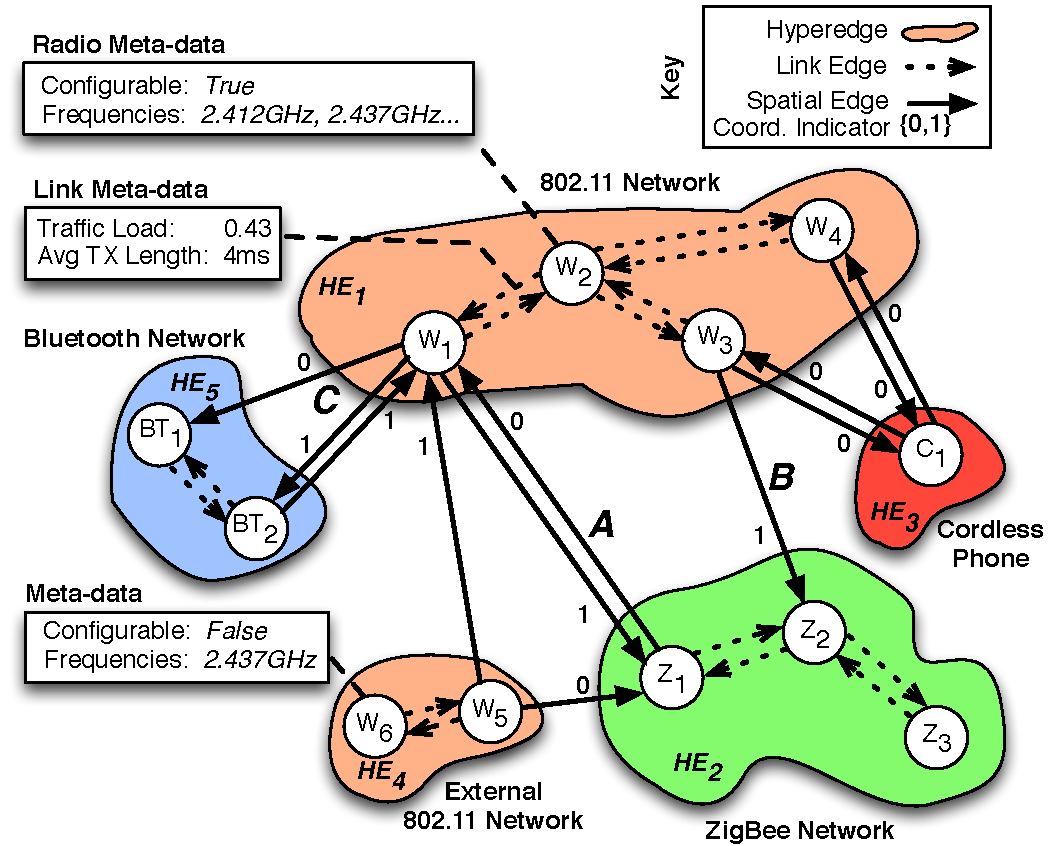
\includegraphics[width=3in]{figures/hypergraph}
\vspace{-0.2in}
\caption{\label{fig:hypergraph} \small Our hypergraph representation of a heterogeneous environment with examples of associated meta-data.}
\center
\vspace{-0.1in}
\end{figure}

\smallskip
\emph{Vertices:} At the base of our hypergraph-model is a set of vertices which represent wireless \emph{radios}.  In todays environments, we believe that it is important to make the base ``unit'' a \emph{radio} for several reasons.  First, networks can span larger areas in which different devices/radios receive different levels of interference.  One cannot assume uniform interference across all radios in a network.  A level lower, devices can have multiple heterogeneous radios (e.g., a laptop with a Bluetooth and Wifi radio), making devices too coarse-grained.  \emph{Radios} truly represent the base unit in today's environments for these reasons.

\smallskip

\emph{Hyperedges:} A hyperedge in our model (e.g., $HE_1$, $HE_2$) represents the network-dependency of wireless radios in the environment, i.e., the radios that form a network and (in spectrum assignment) must be configured uniformly.  For example, we represent this dependency between the three ZigBee radios ($Z_1$, $Z_2$, $Z_3$) which form a network with a hyperedge labeled $HE_2$.    This allows the spectrum assignment model to consider interference at the radio level, accounting for radios in a network which can experience vastly different interference.  Spectrum assignment can then use such a model to minimize interference across the entire network.


%For example, referring to Figure~\ref{fig:hypergraph}, when the link $LE\{W1,W2\}$ is active, $LE\{Z2,Z1\}$ can be impacted since $Z1$ is within spatial range of $W1$

\smallskip
\emph{Edges:}  There are two types of (regular) edges in our model:  1) \emph{Link edges} that explicitly model one-way communication between radios (also implying spatial overlap), and 2) \emph{Spatial edges} that explicitly model spatial overlap between radios in the environment, in addition to whether the overlap causes the opposing radio to back-off (e.g., via energy sensing) using weights.  Link edges should only exists between radios that are connected by a hyperedge (i.e., radios create links within a network),  whereas spatial edges can ``connect" any pair of radios in the environment.   For the purpose of spectrum assignment, however, we do not draw spatial edges within a network (i.e., within a hyperedge). This assumes connectivity and coordination within a network, remaining agnostic to problems such as range issues which (towards our goal) spectrum assignment cannot solve.  

%Since one cannot assume coordination, range, or the symmetry of such properties in heterogeneous environments (e.g., asymmetric coordination is possible~\cite{buzz buzz}), we make 

Critical to a heterogeneous environment, we make spatial edges uni-directional and weight them to represent coordination (a key requirement).  If radio $Y$ is within range of radio $X$, we place a place a uni-directional spatial edge from $X$ to $Y$ denoted $SE\{X,Y\}$.  If active transmissions from $X$ cause $Y$ to back-off, then we weight $SE\{X,Y\}=1$ (0 otherwise).  Together, uni-directionality and coordination weights allow the graph to (importantly) represent asymmetric coordinated behavior (as observed in prior work~\cite{buzz buzz}).  Referring the reader to the edges labeled $A$ in our example, both radios ($Z_1$ and $W_1$) overlap with each other spatially.  However, only the ZigBee radio $Z_1$ backs off to the Wifi node (i.e., $SE\{W_1,Z_1\}$=1), and not visa-versa (i.e., $SE\{Z_1, W_1\}$=0).

We also consider link edges to be uni-directional, where communication from $X$ to $Y$ is denoted $LE\{X,Y\}$.  Considering links as uni-directional is important to properly model interference, best explained through example.  Referring to Figure~\ref{fig:hypergraph}, when the link $LE\{W_1,W_2\}$ is active, $LE\{Z_2,Z_1\}$ can be impacted since the receiver $Z_1$ is within spatial range of $W_1$, which does not back-off to $Z_2$.  However, the ZigBee link in the reverse direction $LE\{Z_1,Z_2\}$ is not impacted by $LE\{W_1,W_2\}$ since there is no spatial edge from the potential interferer $W_1$ to the receiver in this direction: $Z_2$. Uni-directional link edges ensure capturing such behavior.

%$SE\{W_1,Z_2\}$, meaning when $Z_2$ is the receiver (instead of $Z_1$), communication between $Z_1$ and $Z_2$ will not be interrupted by $W_1$ (the transmitter on $LE\{W_1,W_2\}$). 


%\smallskip
%\emph{Link Edges:}  Edges in our model that are embedded within hyperedges are always considered link edges.  These edges are uni-directional and represent communication (i.e., a wireless link) between two radios in the environment.  We denote a link from $W_1$ to $W_2$ as $LE\{W_1,W_2\}$.  Considering such links as uni-directional allows us to properly model interference that a radio can have on specific links, which is sensitive to which radios in the link are the receive and transmitter.  We will provide an example of this in \S\ref{sec:hyperex}.
%
%\smallskip
%\emph{Spatial Edges \& Weights:}  Edges in our model that cross hyperedges are always considered spatial edges.  These edges are similar to those in more traditional models which represent spatial overlap.  However, critical to a heterogeneous environment these edges must be uni-directional to capture the strong asymmetry found between heterogeneous technologies.  We represent a uni-directional edge from vertices $X$ to $Y$ as $SE\{X,Y\}$.  In addition to this uni-directionality, we place a binary weight on each edge (1 or 0) to represent coordination (a key requirement).  Together, uni-directionality and weights allow the graph to (importantly) represent asymmetric coordinated behavior.  For example, we refer the reader to the edges labeled $A$ in our example.  In this scenario, both radios ($Z_1$ and $W_1$) overlap with each other spatially.  However, only the ZigBee radio $Z_1$ backs off to the Wifi node (i.e., $SE\{W_1,Z_1\}$=1), and not visa-versa (i.e., $SE\{Z_1, W_1\}$=0). For the purpose of modeling our environment, we \emph{only} draw edges between vertices (i.e., radios) that are \emph{not} connected by a hyperedge.  This makes the model agnostic to range and/or connectivity issues within a network; assuming within a network there is connectivity.  However, one \emph{could} draw edges between such vertices which, for diagnostics, could illustrate range issues.  

\smallskip
\emph{Meta-data:}  Towards proper configuration during spectrum assignment and a heterogeneous-aware estimation of channel performance (\S\ref{sec:hce}), we annotate each radio and link with a small amount of meta-data.  Radio meta-data can include whether the radio is configurable (e.g., does it belong to the owner's envnironment, or is it an external and neighboring radio?), as well as the supported frequencies of the device.  Note that it may not be possible to know all of the frequencies supported by external radios, however, this information is \emph{not} necessary.  Since such external radios cannot be reconfigured, the only frequency that matters is the radio's current operational frequency, which will be used by the spectrum assignment algorithm.  Link meta-data includes the traffic load (i.e., airtime estimate) of the link and the average transmission length on the link which we later show is important towards estimating interference between radios and links (\S\ref{sec:sigma}).  

%With these remaining pieces of information, we are able to provide a model which meets all of the requirements (\S\ref{sec:requirements}).

\smallskip
\subsubsection{Other Examples in Our Hypergraph Model}  
\label{sec:hyperex}

To further illustrate and describe our model, we refer the reader to two portions of Figure~\ref{fig:hypergraph}.  First, in the section labeled $B$, we show strong asymmetric behavior between $W_3$ and $Z_2$, where $Z_2$ is \emph{not} powerful enough to overlap with $W_3$, however $W_3$ is powerful enough to overlap and cause back-off behavior in $Z_2$.  Additionally, in the set of edges labeled $C$, we show that it is possible to represent two heterogeneous radios that coordinate, e.g., if belonging to the same device, like a Bluetooth and Wifi radio co-located on a laptop.  Here, despite $W_1$ and $BT_2$ being heterogeneous, we can annotate them as being cooperative.  This is unlike $W_1$ and $BT_1$ which are asymmetric and destructive.  
